\newpage
\section{Leitner's Box GUI}
\genHeader
\hypertarget{sec:LBGUI}{}

% Uneeded? We talked a little bit about this in injections.. (it adhgeres to metamodel, or type graph)
We would like to now introduce you to the \texttt{Leitner Box Gui}, a small java application generated from your \texttt{.ecore} instance model! This is the
interface where you can interact with each of your partitions and cards.

\begin{itemize}

\item[$\blacktriangleright$] Navigate to the top left of your toolbar and start the ``New'' wizard.

\item[$\blacktriangleright$] Load ``Examples/eMoflon Handbook Examples/Leitner Box GUI'' (Fig.~\ref{fig:GUI_load}). This will load the new project into
your workspace.\footnote{If nothing appears, go to the small arrow to the right of the window, and select ``Configure Working Sets\ldots'' Make sure
\texttt{Other Projects} is selected, and press \texttt{Ok}} Right click \texttt{LeitnersBox} to raise the context menu and select ``Run as/Java application.''

\begin{figure}[htbp]
    \centering
    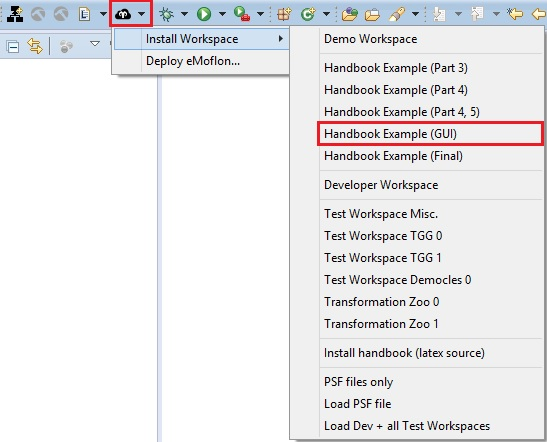
\includegraphics[width=0.7\textwidth]{eclipse_loadGUI}
    \caption{Load Leitner's Box GUI}
    \label{fig:GUI_load}
\end{figure}

\clearpage

\item[$\blacktriangleright$] The GUI will automatically navigate to the instances folder where you've stored your instance model, then load your partitions and
cards into the visualized box.

\vspace{1cm}

\item[$\blacktriangleright$] Navigate to any card, and you'll be able to see two options, ``Remove Card'' and ``Check Card'' (Fig~\ref{fig:GUI_cardOptions}).
While we'll implement ``Check Card" via a different method in Part III, ``Remove Card'' is currently active, completely implemented by the injection you just created.

\vspace{1cm}

\begin{figure}[htbp]
    \centering
    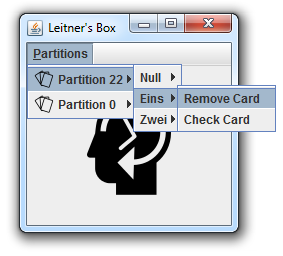
\includegraphics[width=0.5\textwidth]{eclipse_GUICardOptions}
    \caption{Action Options}
    \label{fig:GUI_cardOptions}
\end{figure}

\vspace{1cm}

\item[$\blacktriangleright$] Experiment with your \texttt{.ecore} model and confirm your injection works by removing some items in the GUI.  You'll notice the change immediately in the
``Box.xmi'' tree. You can also close the GUI and try adding, removing, or renaming more attributes in the model itself, then observing how they're reflected
in the window.

% \fancyfoot[R]{ $\triangleright$ \hyperlink{conclusion}{Next}}

\end{itemize}
